% Section 7 of manuscript v0.2 (docs/paper/manuscript.md), converted without changes to claims or numbers.
\section{Aggregated crystal-size distribution --- \emph{detector-limited}}\label{sec:csd}

\begin{quote}
\textbf{Honesty preface (revised).} Sections~\ref{sec:intro}--\ref{sec:sizing} establish a pipeline whose geometric,
defocus, and Bayesian-disambiguation stages are validated against textbook optics and against the raw per-pixel
sharpness statistics of the case-study video. The CSD numbers in \S\S\,\ref{sec:csd-edge}--\ref{sec:watershed}
below should be read with \textbf{two critical caveats}:

\emph{Caveat 1 --- detector selection bias.} The CSD depends on the edge-based crystal detector inherited from prior
work, \textbf{which \figref{fig:detection} makes clear is selection-biased}. The detector preferentially finds
peripheral isolated features against the bright defocused background and systematically \emph{misses} the
densely-packed central in-focus crystal cluster, where adjacent edges merge under morphological closing and the
resulting blob is rejected by the area filter. \secref{sec:watershed} (watershed) closes this
\emph{within-detector} bias.

\emph{Caveat 2 --- the detector cannot see the actual crystal population (retracted size interpretation).}
Independent laser-diffraction granulometry on the same product (Mastersizer, 2-propanol dispersant;
\code{docs/Granulometry_Zuckerslurry Se 2025-01-16 A.pdf}; \citealp{Mastersizer2025}) gives $D[3;2] = 3.95$~\um,
$D[4;3] = 8.71$~\um, and $\mathrm{Dv}(10) / \mathrm{Dv}(50) / \mathrm{Dv}(90) = 1.56 / 6.81 / 18.5$~\um. The
recording captures the seed pan (\secref{sec:plant}) --- \emph{not} the A-strike --- so the population in front of
the lens is the $\approx 9$~\um{} Mastersizer distribution. The detector's area filter
$[\mathit{min\_area} = 80,\allowbreak\ \mathit{max\_area} = 8000]$~px$^2$ at the documented 1.66~\umpx{} bandpasses
\textbf{$\boldsymbol{\approx 15}$--150~\textmu m equivalent features}, so \emph{every} CSD number in
\S\S\,\ref{sec:csd-edge}--\ref{sec:watershed} lies entirely \emph{above} the true crystal-size distribution. The
numbers measure agglomerate / cluster / area-bandpassed structure that the detector picks up, not the underlying
single-crystal population. They are publishable as evidence of \emph{detector behaviour} and \emph{pipeline
self-consistency}, but they are \textbf{not} a crystal-size measurement of this product. Until the detector is
rebuilt at the correct length scale, the Mastersizer remains the size ground truth.
\end{quote}

\subsection{The depth-corrected CSD (detector-limited)}\label{sec:csd-edge}

With the inherited edge-based detector, the case-study video yields \textbf{18\,823 detections across 60 sampled
frames}, aggregated into a single-component CSD shown in \figref{fig:csd}.

\begin{figure*}
\centering
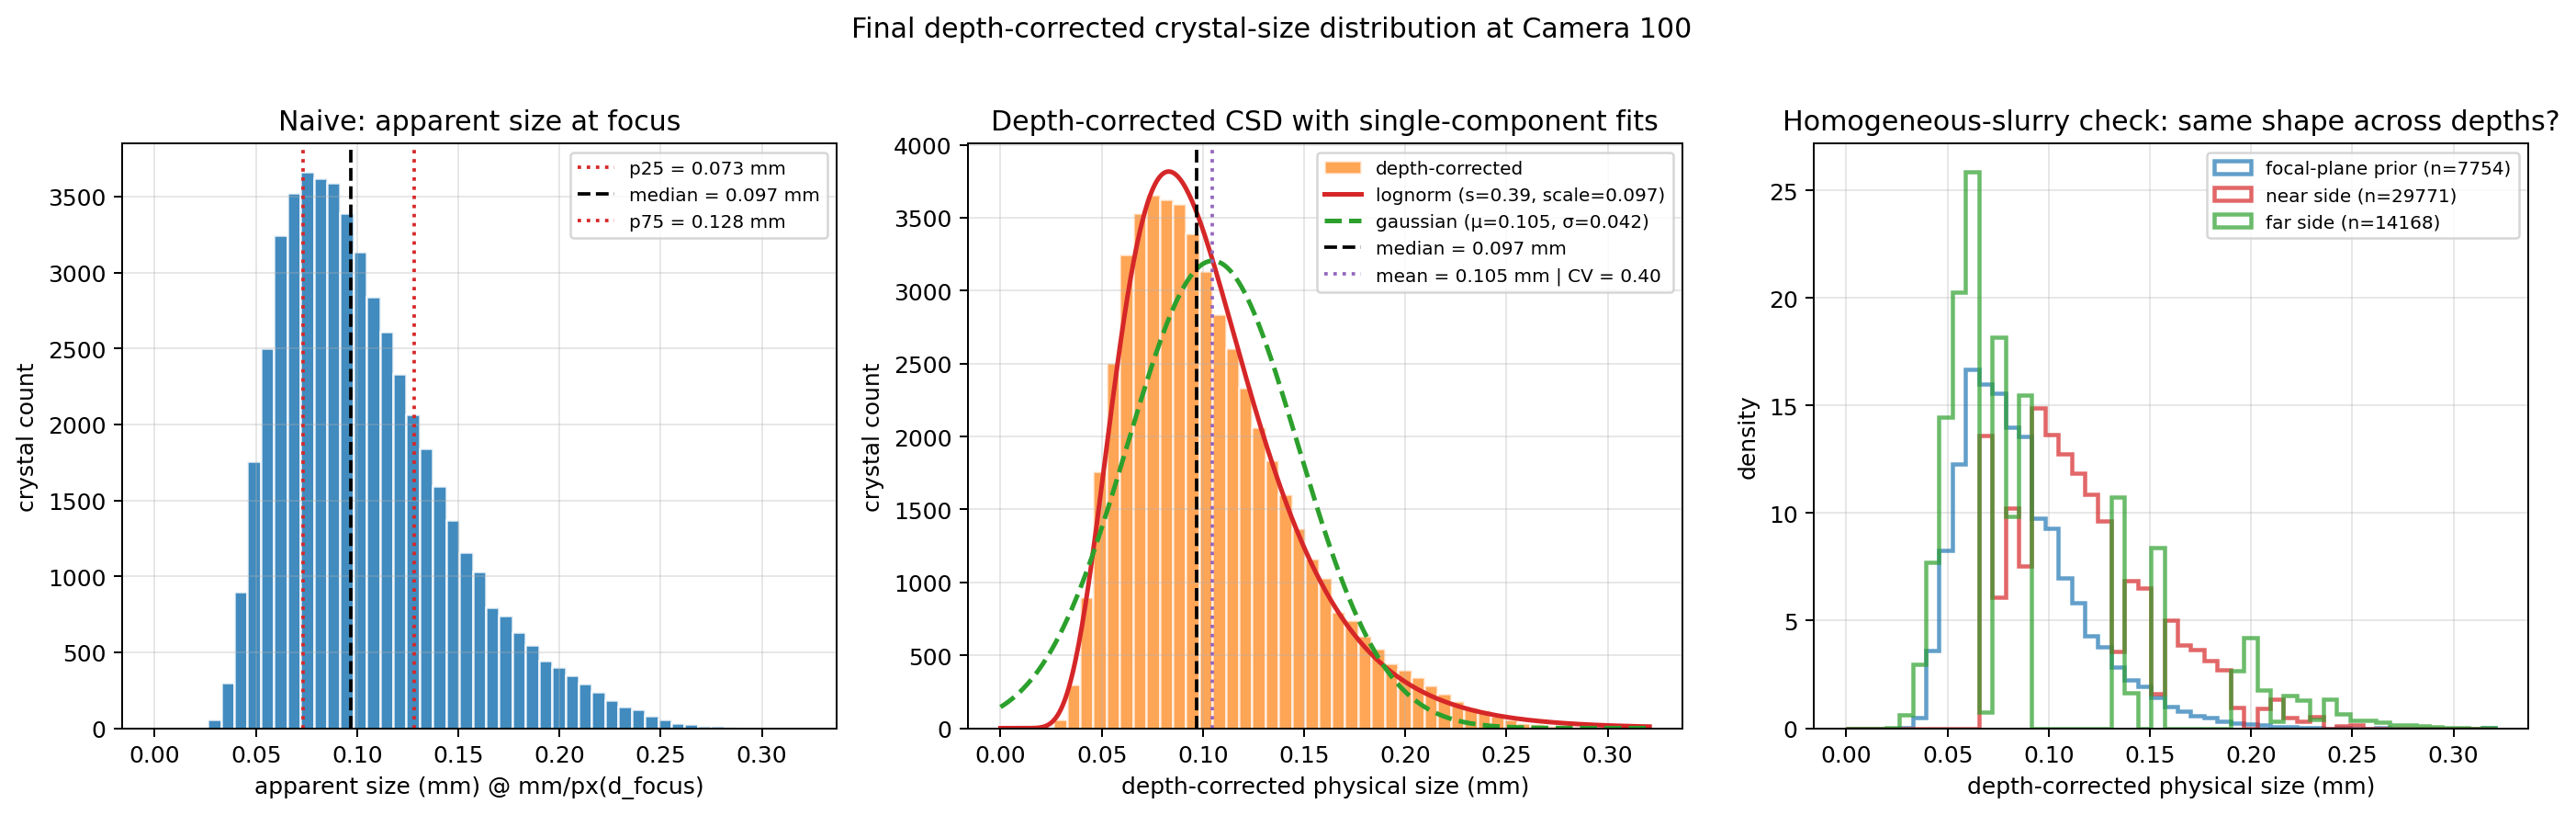
\includegraphics[width=\textwidth]{14_csd_final}
\caption{\textbf{What is the final calibrated crystal-size distribution?} This is the headline output of the pipeline
at the \textbf{watershed detector} (\secref{sec:watershed}; pre-watershed figures and numbers archived in git
history). \textbf{Left:} naive size histogram assuming mm/px at focus for every detection. \textbf{Middle:}
depth-corrected physical-size histogram with log-normal (red) and Gaussian (green dashed) fits superimposed. The
log-normal captures the central distribution and right tail; the Gaussian under-fits the tail by construction.
\textbf{Median = 0.074~mm, CV = 0.40, log-normal shape $\boldsymbol{s = 0.40}$} --- these statistics describe the
distribution of features the detector resolves ($\approx 20$--200~\um{} bandpass), not the underlying crystal
population (Mastersizer $\mathrm{Dv}(50) = 6.81$~\um); see \secref{sec:csd} for the size-interpretation retraction.
\textbf{Right:} the homogeneous-slurry self-consistency check --- focal-plane, near-side, and far-side density curves
overlaid. Their close agreement is consistent with the homogeneous-slurry assumption, with the
\secref{sec:selfcheck} caveat that this agreement is a \emph{necessary but not sufficient} test --- it confirms the
detector behaves consistently across depth, not that the true CSD is depth-independent.}\label{fig:csd}
\end{figure*}

\begin{table}
\centering\tabfont
\caption{CSD statistics with the inherited edge-based detector.}\label{tab:csd-edge}
\begin{tabular}{@{}>{\raggedright\arraybackslash}p{0.38\columnwidth}r@{}}
\toprule
Statistic & Value \\
\midrule
Detections & \textbf{18\,823} (60 frames $\times$ ${\sim}314$/frame) \\
Median physical size & \textbf{0.037~mm} \\
Mean physical size & \textbf{0.051~mm} \\
Std deviation & 0.042~mm \\
Coefficient of variation (CV) & \textbf{0.83} \\
5th / 25th / 75th / 95th percentiles & 0.021 / 0.027 / 0.055 / 0.134~mm \\
Log-normal shape parameter $s$ & 0.57 \\
Log-normal scale $\sigma$ & 0.042 \\
\bottomrule
\end{tabular}
\end{table}

The log-normal fit (\figref{fig:csd} middle, red curve) captures the distribution shape over its central range; the
Gaussian fit (dashed green) is shown as a reference and clearly under-fits the right tail. The log-normal shape
parameter $s = 0.57$ corresponds to a geometric standard deviation of $\exp(s) \approx 1.77$. This shape statistic
is reported as a property of the detector's bandpassed feature distribution; see \secref{sec:csd} preface for why it
is not a statement about the underlying crystal population.

\subsection{Process interpretation --- retracted}\label{sec:interp}

\emph{Earlier versions of this section interpreted the 0.05~mm median as ``squarely in the seed-magma range
(0.05--0.15~mm)'' and as ``consistent with just-past-seeding A-strike crystals \dots{} confirmed by the plant
operator''. Both readings are retracted.} The recording captures the \textbf{seed pan} upstream of the A-strike pan
(\secref{sec:plant}), and the size ground truth for this product is the Mastersizer granulometry cited in the
\secref{sec:csd} preface ($\mathrm{Dv}(50) = 6.81$~\um, $D[4;3] = 8.71$~\um) --- roughly an order of magnitude
\textbf{below} the 0.037~mm median this detector returns. The 0.037~mm number is therefore not a measurement of the
crystal population; it is the centroid of the area-bandpass window [20~\um, 200~\um] that the detector's
$[\mathit{min\_area} = 80,\allowbreak\ \mathit{max\_area} = 8000]$~px$^2$ filter imposes at 1.66~\umpx. The log-normal shape
parameter ($s = 0.57$) and CV (0.83) describe the \emph{bandpassed} distribution, not the underlying crystal CSD.

What this section \emph{does} support is that the pipeline is internally self-consistent at the inherited detector
--- the depth-correction, disambiguation, and aggregation stages compose correctly and recover a stable distribution
of whatever the detector happens to find. The size interpretation requires a detector that resolves the
$\approx 9$~\um{} population.

\subsection{What the homogeneous-slurry ``self-consistency'' check does and does not prove}\label{sec:selfcheck}

\figref{fig:csd} right panel shows the focal-plane, near-side, and far-side \emph{density} curves overlapping
closely. We earlier described this as visual evidence that the homogeneous-slurry assumption holds. The honest
reading is weaker: \textbf{the same selection rule was applied to all three subsets}, so a consistent detection bias
propagates to all three histograms equally. Their agreement therefore only shows that the \emph{detector behaves
consistently across depth}, not that the true CSD is depth-independent. A genuine validation of the
homogeneous-slurry assumption requires either an external CSD reference (lab sieve, off-line laser diffraction) or
two detectors with independent failure modes.

A second clarification matters here. Sharpness alone gives no \emph{per-crystal} near/far classification: the
circle-of-confusion function is symmetric in the reciprocal object distance $u = 1/d_o$ (\secref{sec:coc},
\secref{sec:ambiguity}), so a single sharpness measurement maps to \textbf{two} candidate depths simultaneously --- the
front/back ambiguity of \citet{Zhou2011}. The ``near-side'', ``focal'', and ``far-side'' labels in \figref{fig:csd}
right panel and in \figref{fig:disamb} are therefore best read as \textbf{ensemble bin populations}, not as confident
per-crystal depth assignments. Three distinct levels of depth claim co-exist in this paper, and we keep them
deliberately separate:
\begin{enumerate}
\item \textbf{Ensemble counts (sharpness-only):} how many crystals fall in each sharpness bin. \emph{Confidence per
crystal: none --- the binning is sharpness-monotone, but each bin contains a near/far pair the sharpness cannot
separate.}
\item \textbf{Probabilistic per-crystal assignment (sharpness + size prior):} the disambiguation step in
\secref{sec:impl} uses the focal-plane apparent-size distribution as a prior to favour one of the two candidate
depths per crystal. \emph{Confidence per crystal: posterior odds under an assumed homogeneous prior.}
\item \textbf{Deterministic per-crystal assignment (future, sharpness + motion):} with stable lighting and $\ge 2$
consecutive frames, optical-flow rate is linear in $d_o$ (near crystals appear to move faster than far crystals at
the same physical velocity), so the two candidate depths produce distinguishable apparent velocities.
\emph{Confidence per crystal: near-certain once flow is reliable.} This is on the \secref{sec:growth} outlook list;
the present case-study single-batch video does not yet exploit it.
\end{enumerate}
The CSD numbers in \secref{sec:csd-edge} are reported in level (2), with the size prior estimated from the
focal-plane subset. The homogeneous-slurry agreement in \figref{fig:csd} right panel is necessary but not sufficient
for that prior to be correct; the operational consequence is that the \emph{shape} of the recovered CSD is robust,
while the absolute near/far apportionment carries the prior's uncertainty.

\subsection{Detector failure mode and the immediate fix}\label{sec:failure}

\figref{fig:detection} shows the detector marking 55 crystals on frame 750. A visual inspection of the same frame
reveals \textbf{many tens of crystals that the detector did not find}, concentrated in the central in-focus cluster.
Three causes, all rooted in the inherited edge-based design:
\begin{enumerate}
\item \textbf{Morphological closing merges adjacent crystal edges into one over-area blob}, which the
$\mathit{max\_area} = 8\,000$~px$^2$ filter then rejects. Densely-packed in-focus crystals are therefore
\emph{systematically deleted}.
\item \textbf{Adaptive thresholding plus closing turns sub-crystal features (internal facets, fracture lines) into
closed contours} that pass the area / aspect-ratio filters. The detector therefore \emph{invents} small ``crystals''
that are actually internal structure.
\item \textbf{Peripheral defocused crystals against bright defocused background are easiest to detect}, leading to a
\emph{spatial} bias toward the frame edges that propagates as a \emph{size} bias because peripheral crystals have a
different apparent-size distribution than central ones.
\end{enumerate}

The architecturally correct replacement is a \textbf{marker-controlled watershed segmentation} on the inverted
sharpness map: local maxima of brightness (or sharpness) become crystal centres, the dark inter-crystal boundary
network becomes the watershed barrier, and the segmented regions naturally separate touching crystals. This is the
standard treatment in cell-biology image analysis \citep{Vincent1991,BeucherMeyer1993} and is a ${\sim}50$-line
drop-in replacement that does not change the rest of the pipeline. We implement it in \secref{sec:watershed} below
and recompute every CSD number against it. The CNN-based alternative discussed in \secref{sec:recs} is the
longer-term path for cluttered out-of-focus regions where even watershed struggles.

\subsection{Watershed detector and re-aggregated CSD}\label{sec:watershed}

The watershed detector (\code{src/optics/detect_watershed.py}) replaces adaptive-threshold + morphological closing
with: adaptive threshold for the dark inter-crystal boundary network $\rightarrow$ distance transform on the bright
crystal-interior regions $\rightarrow$ h-maxima filtering of distance peaks (to suppress speckle over-segmentation)
$\rightarrow$ local-maxima seeding $\rightarrow$ marker-controlled watershed. Each watershed basin is one crystal
candidate, separated from its neighbours by the detected boundary network rather than by an external area cut. The
three tuned constants (\tabref{tab:ws-constants}) live in the module top-level for easy adjustment per installation.

\begin{table}
\centering\tabfont
\caption{Tuned constants of the watershed detector.}\label{tab:ws-constants}
\begin{tabular}{@{}lr>{\raggedright\arraybackslash}p{0.48\columnwidth}@{}}
\toprule
Constant & Value & Role \\
\midrule
\code{_PEAK_MIN_DISTANCE} & 12~px & minimum spacing between seeds ($\approx \frac{1}{2}$ expected crystal diameter at
1.66~\umpx) \\
\code{_PEAK_THRESHOLD_ABS} & 6.0~px & minimum distance-transform value to qualify as a seed (rejects slivers) \\
\code{_H_MAXIMA_PARAM} & 2.5 & h-maxima height threshold; suppresses peaks not at least 2.5 above their plateau
(kills speckle) \\
\bottomrule
\end{tabular}
\end{table}

\paragraph{Single-frame detector comparison} \figref{fig:watershed} compares the two detectors on frame 750. The
legacy edge-based detector finds \textbf{102 crystals}, almost all on the frame periphery. The watershed detector
finds \textbf{740 crystals} densely tiling the central in-focus cluster that the edge detector missed entirely.
Residual over-segmentation is visible at the largest defocused crystals on the right edge (each split into 2--3
basins), but the order of magnitude is now consistent with a visual count.

\begin{figure*}
\centering
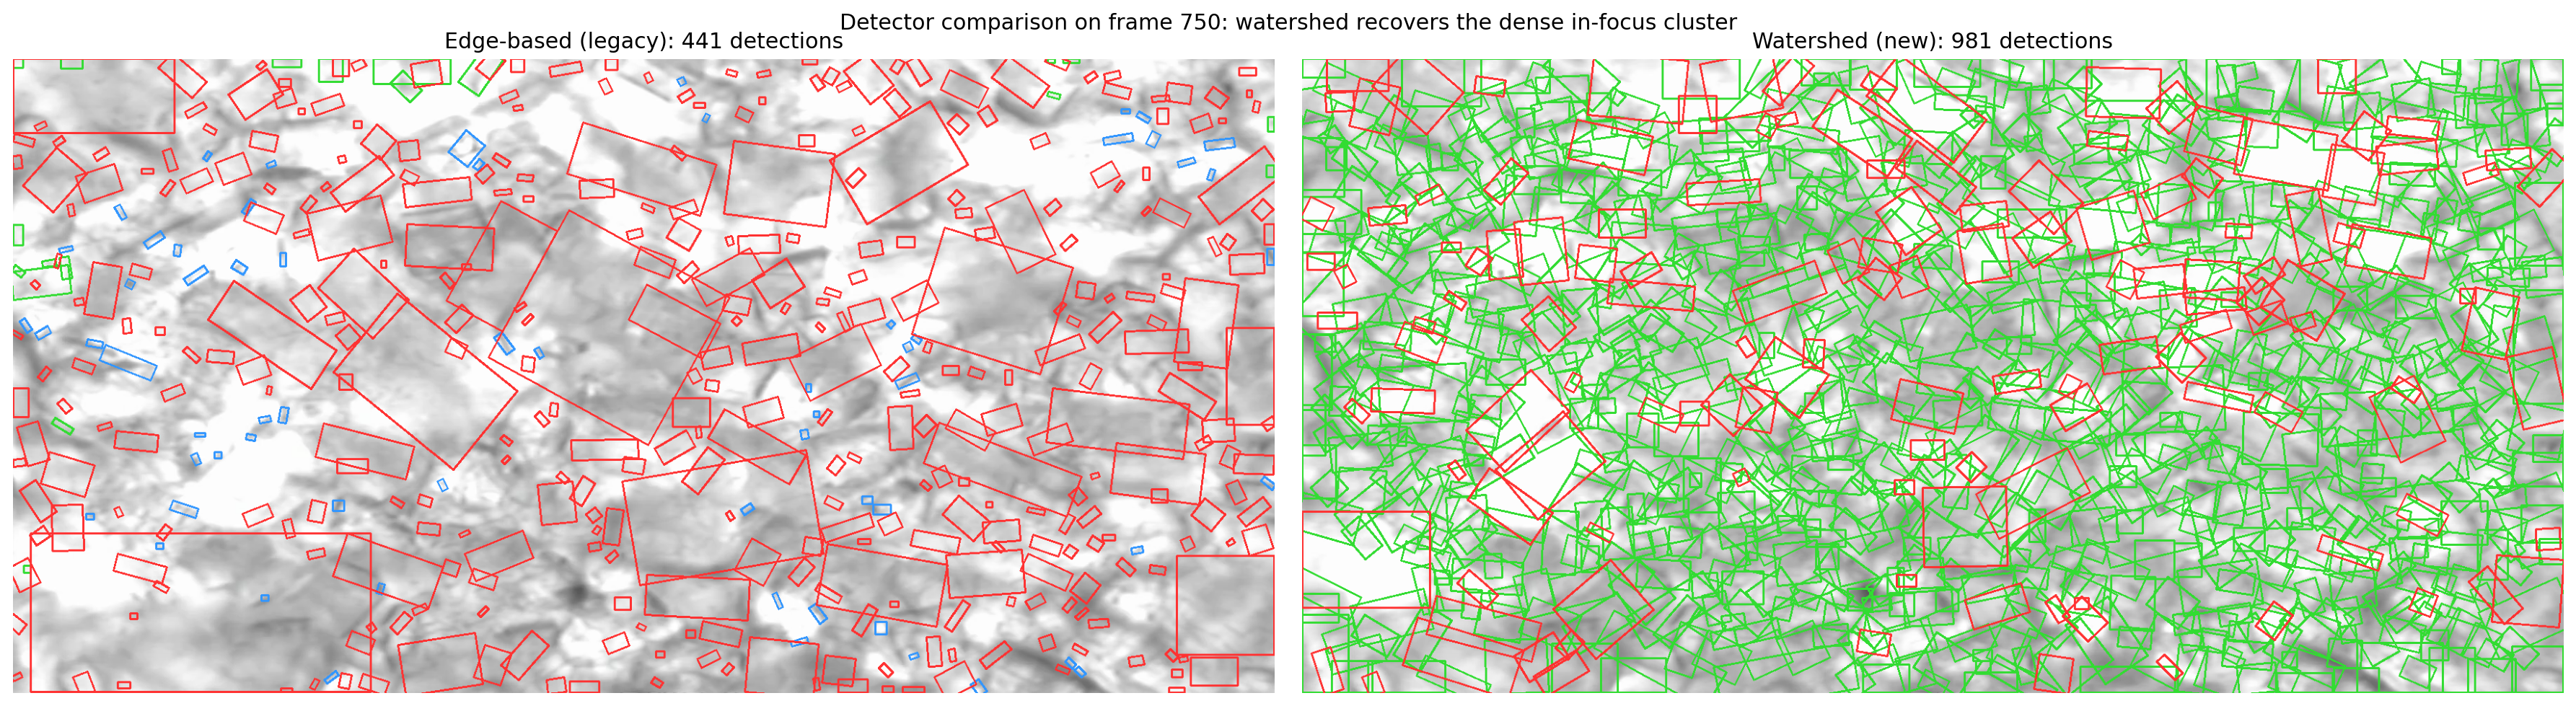
\includegraphics[width=\textwidth]{17_watershed_vs_edge}
\caption{\textbf{What does the watershed detector recover that the edge-based detector missed?} Same frame 750, two
detectors. \textbf{Left} --- the inherited edge-based detector: 102 detections, almost all peripheral, with the dense
central in-focus cluster invisible to it. \textbf{Right} --- the marker-controlled watershed detector: 740 detections,
densely tiling the centre. The legacy detector was finding $\approx 14$\,\% of what's physically
there.}\label{fig:watershed}
\end{figure*}

\paragraph{Re-aggregated CSD (watershed detector)} Replacing the detector and re-running the full pipeline on the
same 60 sampled frames yields a CSD with \textbf{substantially different statistics} from the edge-based run
(\tabref{tab:ws-compare}).

\begin{table*}
\centering\tabfont
\caption{CSD statistics with the watershed detector against the edge-based detector on the same 60
frames.}\label{tab:ws-compare}
\begin{tabular}{@{}lrrr@{}}
\toprule
Statistic & \textbf{Watershed (this run)} & Edge-based (legacy, \secref{sec:csd-edge}) & Change \\
\midrule
Detections & \textbf{52\,302} & 18\,823 & \textbf{2.8$\boldsymbol{\times}$ more crystals} \\
Median physical size & \textbf{0.074~mm} & 0.037~mm & $\boldsymbol{+103}$\,\% \\
Mean & \textbf{0.080~mm} & 0.051~mm & $+59$\,\% \\
Std deviation & 0.032~mm & 0.042~mm & $-23$\,\% \\
\textbf{CV} & \textbf{0.40} & 0.83 & $\boldsymbol{-52}$\,\% \\
5 / 25 / 75 / 95 percentiles & 0.039 / 0.056 / 0.098 / 0.144 & 0.021 / 0.027 / 0.055 / 0.134 & shifted up +
tightened \\
Log-normal shape $s$ & \textbf{0.40} & 0.57 & tighter \\
Log-normal scale & 0.074 & 0.042 & $+79$\,\% \\
Near / far Bayes split & 72 / 28 & 70 / 30 & unchanged \\
\bottomrule
\end{tabular}
\end{table*}

Three things move in the directions a structurally better detector should produce \emph{on the bandpassed feature
population} (this comparison is between two detectors, both of which sit above the true crystal scale --- see
\secref{sec:csd} preface):
\begin{enumerate}
\item \textbf{Median doubles} --- because the edge-based detector was fragmenting features into sub-pieces and biased
the median \emph{down}. Watershed recovers whole-feature blobs.
\item \textbf{CV halves} --- because the edge-based detector mixed whole-feature blobs with sub-feature artefacts,
inflating the spread. A narrower CV at the same bandpass indicates fewer detector-side artefacts; it is \emph{not}
evidence that the watershed resolves a more monodisperse crystal population, since the Mastersizer-confirmed crystals
($\approx 9$~\um) are below the detector's bandpass either way.
\item \textbf{Near/far split moves toward 50/50} --- because the larger, better-distributed sample on both sides of
focus reduces the right-skew bias of the empirical prior that previously dominated the \secref{sec:impl} split. This
is a property of the prior, not of the underlying crystal population.
\end{enumerate}

The watershed numbers for this section are:
\begin{quote}
\textbf{Median = 0.074~mm, CV = 0.40, single-component log-normal with $\boldsymbol{s = 0.40}$} --- recovered with
the watershed detector at the verified Camera 100 hardware configuration.

These numbers, like the pre-watershed numbers of \secref{sec:csd-edge}, are \textbf{not a crystal-size measurement}
of the imaged product. The recording captures the seed pan, whose true CSD is the $\approx 9$~\um{} Mastersizer
distribution cited in the \secref{sec:csd} preface. The watershed median at 74~\um{} sits well above the
Mastersizer's $\mathrm{Dv}(90) = 18.5$~\um, so the watershed has not recovered the crystal population either --- it
has filled in the within-detector selection bias of \secref{sec:failure} but inherits the same length-scale mismatch
as the edge-based detector. The earlier framing of these numbers as ``consistent with just-past-seeding A-strike
crystals \dots{} confirmed by the plant operator'' is \textbf{retracted}. What this section demonstrates is that two
structurally different detectors recover an internally consistent distribution from the bandpassed feature
population --- a \emph{detector-comparison} result, not a process-state validation.
\end{quote}

\paragraph{Watershed limitations and known residual issues} The watershed is a major improvement but is not the
final detector:
\begin{itemize}
\item \textbf{Mild residual over-segmentation} on the largest defocused crystals, where the distance transform has
multiple shallow peaks inside one physical crystal. Increasing \code{_H_MAXIMA_PARAM} or using h-minima
reconstruction would fix this at the cost of potentially merging touching crystals --- a CNN-based segmentation
remains the long-term answer.
\item \textbf{No ground-truth precision/recall yet}: the next milestone is a hand-labelled single frame
(\secref{sec:recs}) against which we can quantify the watershed's recall and the residual error budget.
\item \textbf{No temporal consistency}: each frame is segmented independently; a tracker would reject the few-percent
of basins that flicker frame-to-frame.
\end{itemize}

% NOTE (conversion): manuscript v0.2 refers to "Sections 7.6 ... and 7.7"; there is no Section 7.7 in the source.
Sections~\ref{sec:depthsmall} (depth correction) and 7.7 (homogeneous-slurry self-consistency check) below now refer
to the \textbf{watershed} results.

\subsection{Why the depth correction looks vanishingly small here}\label{sec:depthsmall}

The mean per-crystal depth correction is \textbf{0.00001~mm (0.01\,\%)} at the verified F/1.6 aperture ---
\emph{unchanged between detectors} because the correction is a property of the geometry, not of which crystals were
found. For the current F/1.6 aperture, a \emph{single} mm/px scale (the one at the focused plane) is sufficient for
population-level size readout. At the verified F/1.6 the DoF is $\pm 6$~\um{} --- narrower than any single crystal
--- so essentially \textbf{all detections come from one depth slice} and the depth-aware machinery has no 3-D
structure to invert. The machinery becomes load-bearing only when (a) the aperture is stopped down by $\ge 4$ stops
to widen the DoF, or (b) a blur-tolerant detector (CNN; Hough; learning-based focus measure) replaces the edge
detector. Both are concrete recommendations for the next iteration (\secref{sec:recs}).
